\section*{جواب سوال ۲}

جواب این سوال می‌تواند خیلی طولانی باشد و با بررسی نکات مختلف هر کدام از امکان‌سنجی‌ها، اما تلاش می‌کنم به شکل خلاصه جواب دهم به هر کدام از سوالات.

\section{بررسی امکان‌سنجی}
\subsection{امکان‌سنجی فنی}
امکان‌سنجی فنی به ارزیابی توانایی فنی سازمان برای توسعه پروژه می‌پردازد. این بررسی شامل تحلیل زیرساخت‌های موجود، دانش فنی تیم، و تکنولوژی‌های لازم است. در واقع سوال آیا می‌توانیم بسازیم را در این‌جا جواب می‌دهیم.

\textbf{ریسک‌ها:}
\begin{itemize}
	\item \textit{کمبود دانش فنی:} اگر تیم توسعه دانش کافی راجع به تکنولوژی‌های جدید نداشته باشد، پروژه ممکن است با شکست مواجه شود.
	\item \textit{محدودیت‌های زیرساختی:} زیرساخت‌های ناکافی می‌تواند مانعی برای پیاده‌سازی موفق پروژه باشد.
\end{itemize}

\textbf{راه حل‌ها:}
\begin{itemize}
	\item برای کمبود دانش فنی، برنامه‌ریزی دوره‌های آموزشی و کارگاه‌های تخصصی پیشنهاد می‌شود.
	خیلی وقت‌ها این مورد رو با استخدام کارشناسان به‌خصوص و متخصص در زمینه‌های مختلف نیز بهبود می‌دهند و این مشکل را حل می‌کنند.
	\item برای محدودیت‌های زیرساختی، به‌روزرسانی و ارتقاء زیرساخت‌ها قبل از شروع پروژه ضروری است.
	در این بخش نیاز به بودجه‌ی مالی دقیق و همچنین برنامه‌ریزی درست برای هزینه‌های زیرساختی خواهد بود.
\end{itemize}

\subsection{امکان‌سنجی اقتصادی}
امکان‌سنجی اقتصادی به بررسی صرفه اقتصادی پروژه از جنبه‌های هزینه و سودآوری می‌پردازد. در واقع، در این بخش به سوال آیا باید این پروژه را انجام دهیم می‌پردازیم و جواب این سوال را می‌دهیم.	 گام‌های این سنجش بدین شکل هستند:

۱- شناخت سودها و زیان‌های سیستم

۲- اعطای مقدار به آنان

۳- مشخص ساختن جریان مالی

۴- مشخص ساختن برآیند ارزش فعلی

۵- مشخص ساختن بازگشت روی سرمایه

۶- مشخص ساختن نقطه سرشکن

۷- نمایش نموداری نقطه سرشکن
\newpage

\textbf{ریسک‌ها:}
\begin{itemize}
	\item \textit{هزینه‌های پیش‌بینی نشده:} هزینه‌های غیرمنتظره می‌تواند برآوردهای اولیه را نامعتبر کند.
	\item \textit{تخمین نادرست سود:} بیش‌برآورد کردن سود می‌تواند منجر به تصمیم‌گیری‌های نادرست شود.
\end{itemize}

\textbf{راه حل‌ها:}
\begin{itemize}
	\item برای مقابله با هزینه‌های پیش‌بینی نشده، ایجاد یک بودجه احتیاطی توص
	یه می‌شود.
	\item برای جلوگیری از تخمین نادرست سود، انجام تحلیل‌های بازار دقیق‌تر و استفاده از داده‌های تاریخی مشابه برای پیش‌بینی‌های واقع‌بینانه توصیه می‌شود.
\end{itemize}

\subsection{امکان‌سنجی سازمانی}
امکان‌سنجی سازمانی به ارزیابی تطابق پروژه با اهداف و استراتژی‌های کلی سازمان می‌پردازد. در واقع به سوال اگر بسازیم آیا سرمایه‌گذاران می‌آیند این‌جا پاس می‌دهیم. به‌خصوص باید بررسی کنیم هم‌سو هستش اهداف پروژه با اهداف کسب و کار روزمره یا خیر.

\textbf{ریسک‌ها:}
\begin{itemize}
\item \textit{مقاومت در برابر تغییر:} کارکنان ممکن است نسبت به تغییرات ناشی از پروژه مقاومت نشان دهند.
\item \textit{ناهماهنگی با اهداف سازمانی:} پروژه ممکن است با اهداف بلندمدت سازمان هماهنگ نباشد.
\end{itemize}

\textbf{راه حل‌ها:}
\begin{itemize}
\item برای مقابله با مقاومت در برابر تغییر، برگزاری جلسات توجیهی و ایجاد ارتباطات موثر با کارکنان پیشنهاد می‌شود.
\item برای اطمینان از هماهنگی با اهداف سازمانی، باید از مراحل اولیه برنامه‌ریزی، اهداف پروژه با اهداف کلی سازمان مطابقت داده شود.
\end{itemize}

\section{محاسبه سود و زیان پروژه "رندان"}
\subsection{تحلیل سود}

\begin{figure}[H]
	\centering
	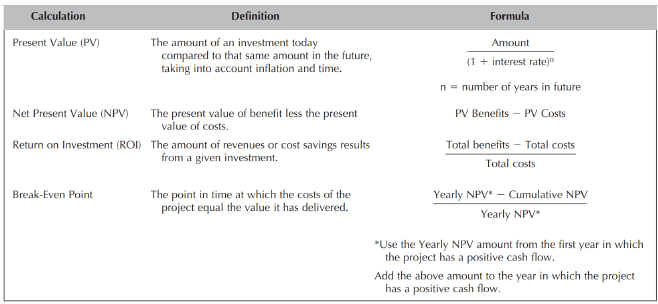
\includegraphics{pic1.jpg}
	
	\label{fig:label4}
\end{figure}

در این عکس، تعاریف هر کدام از موارد مختلف این بخش را می‌بینیم.

برای تحلیل سود پروژه "رندان"، ابتدا با استفاده از داده‌های فروش پیش‌بینی شده توسط مالک محصول و رشد پیش‌بینی شده توسط مدیر مالی، سود خالص هر سال محاسبه می‌شود. سپس، با احتساب سود مازاد حاصل از فروش افزونه‌ها، جمع کل سودهای هر سال به دست می‌آید.

\subsection{تحلیل زیان}
در بخش زیان، هزینه‌های مرتبط با نگهداری سرورها و حقوق کارکنان محاسبه شده و به عنوان هزینه‌های عملیاتی در نظر گرفته می‌شود. همچنین، با توجه به افزایش حقوق سالانه کارکنان، هزینه‌های مرتبط با نیروی انسانی برای هر سال پیش‌بینی می‌شود.

\subsection{محاسبه بازگشت سرمایه و نقطه سر به سر}
بازگشت سرمایه (ROI) با مقایسه کل سود حاصل از پروژه با کل هزینه‌های پروژه محاسبه می‌شود. نقطه سربه سر (BEP)، زمانی را نشان می‌دهد که در آن کل درآمدها با کل هزینه‌ها برابر می‌شوند و پروژه شروع به سوددهی می‌کند. برای محاسبه این دو شاخص، ابتدا باید ارزش فعلی خالص (NPV) و سپس ROI و BEP بر اساس آن محاسبه شود.

\textbf{محاسبه NPV :} NPV با استفاده از نرخ بهره مورد انتظار و جریان‌های نقدی پیش‌بینی شده برای پروژه محاسبه می‌شود. این شاخص به ما می‌گوید که ارزش کل پروژه با توجه به زمان و ارزش زمانی پول چقدر است.

\textbf{محاسبه ROI :} ROI با تقسیم کل سود خالص به دست آمده از پروژه (پس از کسر هزینه‌ها) بر کل سرمایه‌گذاری اولیه (هزینه‌های پروژه) محاسبه می‌شود. این شاخص نشان‌دهنده درصد بازگشت سرمایه از پروژه است.

\textbf{محاسبه BEP :} BEP زمانی را نشان می‌دهد که در آن درآمد حاصل از پروژه برای اولین بار هزینه‌های انجام پروژه را پوشش می‌دهد. این نقطه از نظر زمانی نشان‌دهنده شروع سوددهی پروژه است.

\subsection{نتیجه‌گیری}

\begin{table}[h!]
	\centering
	\begin{tabular}{| m{2cm} | m{2cm} | m{2cm} | m{2cm} | m{2cm} |}
		\hline
		\textbf{محصول} & \textbf{سال سوم} & \textbf{سال دوم} & \textbf{سال اول} & \textbf{فروش محصول} \\
		\hline
		$7275$ & $3150$ & $2625$ & $1500$ & \textbf{فروش محصول} \\
		\hline
		$291$ & $126$ & $105$ & $60$ & \textbf{فروش افزونه‌ها} \\
		\hline
		$7566$ & $3276$ & $2730$ & $1560$ & \textbf{جمع سودها} \\
		\hline
		$6135.4$ & $2461.3$ & $2256.1$ & $1418$ & \textbf{ارزش لحظه‌ای سودها (Present Value)} \\
		\hline
	\end{tabular}
	\caption{جدول سودها؛ مقادیر عددی به واحد میلیون تومان هستند.}
	\label{table:profits}
\end{table}

\begin{table}[h!]
	\centering
	\begin{tabular}{| m{2cm} | m{2cm} | m{2cm} | m{2cm} | m{2cm} |}
		\hline
		\textbf{محصول} & \textbf{سال سوم} & \textbf{سال دوم} & \textbf{سال اول} & \textbf{حقوق افراد} \\
		\hline
		$7625$ & $3125$ & $2500$ & $2000$ & \textbf{فروش محصول} \\
		\hline
		$250$ & $0$ & $0$ & $250$ & \textbf{نگهداری سرورها} \\
		\hline
		$7875$ & $3125$ & $2500$ & $2250$ & \textbf{جمع زیان‌ها} \\
		\hline
		$6459.3$ & $2347.8$ & $2066.1$ & $2045.4$ & \textbf{ارزش لحظه‌ای زیان‌ها (Present Value)} \\
		\hline
	\end{tabular}
	\caption{جدول زیان‌ها؛ مقادیر عددی به واحد میلیون تومان هستند.}
	\label{table:losses}
\end{table}

در جدول بالا تمامی مفاهیم و فرمول‌های لازم برای این سوال آمده است. اما به جهت شفاف‌سازی به ارائه بررسی کوتاهی از مفاهیم موجود می‌پردازیم.

منظور از 
\textbf{\lr{Present Value}}
یا ارزش فعلی، دخیل کردن فاکتور زمان و مواردی اقتصادی چون تورم، سود و \ldots می‌باشد چرا که با در نظر گرفتن این موارد، ارزش دلار امروز با ارزش دلار فردا برابر نمی‌باشد.

منظور از 
\textbf{\lr{Return on Investment (ROI)}}
یا بازگشت سرمایه، به معنای محاسبه سود کلی سازمان و دخیل کردن ضررها و سرمایه‌گذاری‌ها در کنار سودها می‌باشد و در انتها نیز مقدار این تفریق دوباره تقسیم بر کلیه هزینه‌ها معمولا به صورت سالانه و یا پروژه محور صورت می‌گیرد. مشکل این معیار عدم در نظر گرفتن وضعیت مالی در سازمان در بازه‌های کوتاه مدت می‌باشد و نمی‌تواند به تنهایی نشان‌گر وضعیت مالی پروژه باشد.

بازگشت سرمایه در این پروژه برابر مقدار زیر می‌باشد:
\[
\frac{(7566 - 7875)}{7875} = -0.039
\]

مفهوم 
\textbf{\lr{Break Even Point (BEP)}}
نیز به معنای نقطه‌ای است که میزان سود سازمان با ضررها و سرمایه‌گذاری‌های صورت گرفته در آن برابر می‌شود. با توجه به اهمیت عنصر زمان در این معیار لازم است که از 
\textbf{\lr{Present Value (PV)}} استفاده کنیم. نهایی حاصل تفریق 
\textbf{\lr{Net Present Value (NPV)}} با مجموع \textbf{\lr{NPV}} سالانه (در اولین سالی که روند مالی شرکت مثبت شده است) می‌باشد.

با توجه به مقادیر موجود در نمودارهای ارائه شده (و عدم برخورد نمودار‌های سود و هزینه)، پروژه مذکور در سوال در حدفاصل سه ساله به نقطه \textbf{BEP} نمی‌رسد.